\chapter{Background}

In this chapter we introduce some general notions as well as a more deep understanding of what P systems and Petri nets are.

\section{Basic Definitions}

\begin{definition}[Multiset]
Let $U$ be an arbitrary set. A multiset over U is a mapping \newline $m : U \rightarrow N$.
The multiplicity of an element $u$ in $m$ is given by the natural number $m(s)$.
\end{definition}

\begin{definition}[Alphabet]
An alphabet is a finite nonempty set of abstract symbols. Given an alphabet $V$, we denote by $V^*$
the sets of all finite strings of elements in $V$, including the empty string $\lambda$.
Every string $v \in V$ describes a multiset over $V$.
\end{definition}

\section{P Systems}

Membrane computing is a branch of natural computing, introduced by Gheorghe Paun with the definition of P systems in \cite{puaun2000computing,puaun2002membrane,paun1999computing}.

Membrane systems are based upon the notion of \textit{membrane structure}, which is a structure composed by several cell-membranes, hierarchically embedded in a main membrane called the \textit{skin membrane}.
The membranes delimit \textit{regions} and we associate with each region a set of \textit{objects}, described by some symbols over an alphabet, and a set of \textit{evolution rules}.
In the basic variant, the objects evolve according to the evolution rules, which can modify the objects to obtain new objects.
The evolution rules are applied in a maximally parallel manner: at each step, all the objects which can evolve should evolve.
If a computation \textit{halts}, so no further evolution rule can be applied, the result of the computation is defined to be the number of objects in a specified membrane.

\begin{definition}[P system]
A P system (of degree $d$, with $d \geq 1$) is a tuple
\[ \Pi = (V,\mu,w^0_1,...,w^0_d,R_1,...,R_d, i_0)\]
where:
\begin{enumerate}
  \item $V$ is an alphabet; its elements are called objects;
  \item $\mu$ is a membrane structure consisting of $d$ membranes (labeled with $1,2,...,d$);
  \item $w^0_1, 1 \leq i \leq d$, are strings from $V^*$ representing multisets over $V$ associated
  with the regions $1,2,...,d$ of $\mu$;
  \item $R_i, 1 \leq i \leq d$, are finite sets of evolution rules over $V$ associated 
  with the regions $1,2,...,d$ of $\mu$; these evolution rules are of the form $u \rightarrow v$,
  where $u$ and $v$ are strings from $V*$;
  \item $i_0$ is a number between 1 and $d$ which specifies the output membrane of %\Pi;
\end{enumerate}
A configuration of $\Pi$ is a tuple $C=(w_1,...,w_d)$ of multisets of objects, and 
$C_0=(w^0_1,...,w^0_d)$ is the initial configuration.
\end{definition}

According to \cite{agrigoroaiei2010flattening}, any P system can be flattened to a system of degree 1, we call this type of P systems \textit{flat P systems}.
For the sake of simplicity, from now on when we talk about P systems we refer to flat P systems.

\begin{definition}[Flat P system]
A flat P system is a P system of degree one
\[ \Pi = (V,\mu,w^0,R) \]

Given the fact that we're working with a one degree system we removed the subscript from $w$ and $R$. 
A configuration of $\Pi$ is a singleton $C=(w)=w$ of a multiset of objects, and 
$C_0=(w^0)=w^0$ is the initial configuration.
\end{definition}

The following example will clarify the definition of a P system.
Consider the system of degree 1:
\begin{description}
   \item $\Pi=(V,\mu,w^0,R)$,
   \item $V=\{a,b,c\}$,
   \item $\mu=[_{1}]_{1}$,
   \item $C_0=w^0=a^2b$,
   \item $R=\{r_1:a \rightarrow b, r_2:a \rightarrow c\}$
\end{description}

The system is represented in Fig 2.1.

\begin{figure}[h]
\centering

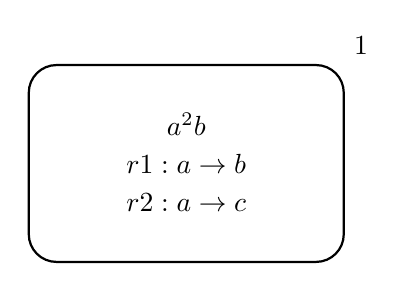
\begin{tikzpicture}
    \draw[thick, rounded corners=10pt] (0, 0) rectangle (4, 2.5) node[above right] {1};
    
    \node at (2, 1.75) {$a^2b$};
    \node at (2,1.25) (rule) {$r1: a \rightarrow b$};
    \node at (2,0.75) (rule) {$r2: a \rightarrow c$};
\end{tikzpicture}

\caption{}
\label{}
\end{figure}

The possibilities to evolve in one step from the initial configuration are: 
\begin{description}
    \item $C=w=b^3$, obtained applying $r=r_1^2$,
    \item $C=w=bc^2$, obtained applying $r=r_2^2$,
    \item $C=w=b^2c$, obtained applying $r=r_1 r_2$
\end{description}

\subsection{Synchronized P systems}

In this section we introduce a new class of P systems, P systems with \textit{synchronization among the rules of the same membrane}.
In the previous section we've seen a kind of synchronization where all regions use their rules in parallel in the maximal mode.
That synchronization that we're interested in is different, more exactly, a rule synchronizing with a non-empty set of rules is applicable at least once only if each rule from the set of rules is applicable at least once.

We call P systems with this kind of synchronization \textit{synchronized P systems}.
They are introduced and talked in \cite{aman2019synchronization,aman2022power}.

\begin{definition}[Synchronized P system]
A synchronized P system is a tuple

\[ \Pi = (V,\mu,w^0,R,\rho) \]

where:
\begin{enumerate}
    \item $(V,\mu,w^0,r)$ is a flat P system;    
    \item $\rho$ is a partial relation defined over the set $R$ of rules specifying
    the synchronization relation over the rules;
    $\rho$ is irreflexive, asymmetric and transitive;
\end{enumerate}
\end{definition}

Let's try to understand better what syncronization means:
let $(r1,r2) \in \rho$; if $r1$ is executed at least one time, then also
$r2$ has to be executed at least one time during this step, and vice versa; if that is not possible neither of them will be executed during the current step.

We use the following notation to describe an instance of $\rho$: 
$\rho=((r1 \otimes r2),(r3 \otimes r4 \otimes r5))$.
This means that $r_1$ can be executed only and only if $r_2$ can be executed at least one time;
in addition, $r_1$ it's executed at least one time only and only if also $r_2$ it's executed at least one time.
Let's see an example to grasp the concept...

\begin{definition}[synchronization rule]
\label{def:sync_rule}
We define a synchronization rule $r_s$ as a set of rules defined by a tuple in $\rho$.
\end{definition}

So given the previous example $(r1 \otimes r2) \in \rho$ then $r_s=\{r1,r2\}$.

\section{Petri Net}

Here we define in a formal way what a Petri Net is.

\subsection{Petri Nets with Inhibitor Arcs}

Here we extend the latter definition of a Petri Net with the concept of inhibitor arcs.